% Options for packages loaded elsewhere
\PassOptionsToPackage{unicode}{hyperref}
\PassOptionsToPackage{hyphens}{url}
%
\documentclass[
  ignorenonframetext,
]{beamer}
\usepackage{pgfpages}
\setbeamertemplate{caption}[numbered]
\setbeamertemplate{caption label separator}{: }
\setbeamercolor{caption name}{fg=normal text.fg}
\beamertemplatenavigationsymbolsempty
% Prevent slide breaks in the middle of a paragraph
\widowpenalties 1 10000
\raggedbottom
\setbeamertemplate{part page}{
  \centering
  \begin{beamercolorbox}[sep=16pt,center]{part title}
    \usebeamerfont{part title}\insertpart\par
  \end{beamercolorbox}
}
\setbeamertemplate{section page}{
  \centering
  \begin{beamercolorbox}[sep=12pt,center]{part title}
    \usebeamerfont{section title}\insertsection\par
  \end{beamercolorbox}
}
\setbeamertemplate{subsection page}{
  \centering
  \begin{beamercolorbox}[sep=8pt,center]{part title}
    \usebeamerfont{subsection title}\insertsubsection\par
  \end{beamercolorbox}
}
\AtBeginPart{
  \frame{\partpage}
}
\AtBeginSection{
  \ifbibliography
  \else
    \frame{\sectionpage}
  \fi
}
\AtBeginSubsection{
  \frame{\subsectionpage}
}
\usepackage{lmodern}
\usepackage{amssymb,amsmath}
\usepackage{ifxetex,ifluatex}
\ifnum 0\ifxetex 1\fi\ifluatex 1\fi=0 % if pdftex
  \usepackage[T1]{fontenc}
  \usepackage[utf8]{inputenc}
  \usepackage{textcomp} % provide euro and other symbols
\else % if luatex or xetex
  \usepackage{unicode-math}
  \defaultfontfeatures{Scale=MatchLowercase}
  \defaultfontfeatures[\rmfamily]{Ligatures=TeX,Scale=1}
\fi
% Use upquote if available, for straight quotes in verbatim environments
\IfFileExists{upquote.sty}{\usepackage{upquote}}{}
\IfFileExists{microtype.sty}{% use microtype if available
  \usepackage[]{microtype}
  \UseMicrotypeSet[protrusion]{basicmath} % disable protrusion for tt fonts
}{}
\makeatletter
\@ifundefined{KOMAClassName}{% if non-KOMA class
  \IfFileExists{parskip.sty}{%
    \usepackage{parskip}
  }{% else
    \setlength{\parindent}{0pt}
    \setlength{\parskip}{6pt plus 2pt minus 1pt}}
}{% if KOMA class
  \KOMAoptions{parskip=half}}
\makeatother
\usepackage{xcolor}
\IfFileExists{xurl.sty}{\usepackage{xurl}}{} % add URL line breaks if available
\IfFileExists{bookmark.sty}{\usepackage{bookmark}}{\usepackage{hyperref}}
\hypersetup{
  pdftitle={Text Mining aplicado ao Projeto HF2},
  pdfauthor={Viviane Schneider},
  hidelinks,
  pdfcreator={LaTeX via pandoc}}
\urlstyle{same} % disable monospaced font for URLs
\newif\ifbibliography
\usepackage{graphicx}
\makeatletter
\def\maxwidth{\ifdim\Gin@nat@width>\linewidth\linewidth\else\Gin@nat@width\fi}
\def\maxheight{\ifdim\Gin@nat@height>\textheight\textheight\else\Gin@nat@height\fi}
\makeatother
% Scale images if necessary, so that they will not overflow the page
% margins by default, and it is still possible to overwrite the defaults
% using explicit options in \includegraphics[width, height, ...]{}
\setkeys{Gin}{width=\maxwidth,height=\maxheight,keepaspectratio}
% Set default figure placement to htbp
\makeatletter
\def\fps@figure{htbp}
\makeatother
\setlength{\emergencystretch}{3em} % prevent overfull lines
\providecommand{\tightlist}{%
  \setlength{\itemsep}{0pt}\setlength{\parskip}{0pt}}
\setcounter{secnumdepth}{-\maxdimen} % remove section numbering

\title{Text Mining aplicado ao Projeto HF2}
\author{Viviane Schneider}
\date{20 de abril de 2020}

\begin{document}
\frame{\titlepage}

\begin{frame}{Contexto do Estudo}
\protect\hypertarget{contexto-do-estudo}{}
O estudo é aplicado no âmbito do Projeto HF2 para obter os seguintes
resultados:

\begin{itemize}[<+->]
\item
  Formular indicadores de coerência de senso de unidade das equipes de
  Libra, a partir de comunicações e story telling descritos no projeto,
\item
  Verificar a aderência dos indicadores do framework de análise do
  projeto em relação à literatura e aos relatórios de acidentes de
  plataformas de óleo e gás.
\item
  Extrair indicadores que permitirão mapear as trilhas das falhas em
  fatores humanos que podem culminar em eventos catastróficos no âmbito
  das plataformas de óleo e gás.
\end{itemize}
\end{frame}

\begin{frame}{O que é Text Mining?}
\protect\hypertarget{o-que-uxe9-text-mining}{}
A Mineração de texto pode ser considerada como sinônimo de descoberta de
conhecimento em textos.

Estes textos que podem ser e-mails; arquivos em diferentes formatos
(pdf, doc, txt, por exemplo); páginas Web; campos textuais em bancos de
dados; textos eletrônicos digitalizados a partir de papéis, etc.

\textbf{Contribuições desta área:}

\begin{itemize}[<+->]
\item
  seleção de documentos,
\item
  classificação de documentos,e
\item
  qualificação de documentos.
\end{itemize}
\end{frame}

\begin{frame}{Etapas do TM}
\protect\hypertarget{etapas-do-tm}{}
\begin{figure}
\centering
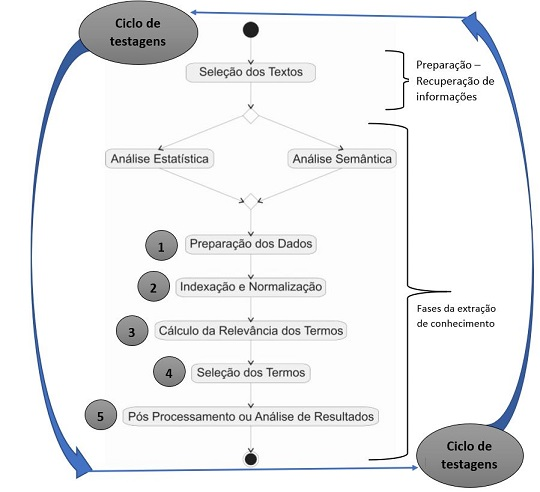
\includegraphics{Fases TM.png}
\caption{Etapas de Text Mining}
\end{figure}
\end{frame}

\begin{frame}{Análise semântica}
\protect\hypertarget{anuxe1lise-semuxe2ntica}{}
Técnicas fundamentadas em Processamento de Linguagem Natural (PNL), que
avaliam a seqüência dos termos no contexto dos textos. Necessita dos
seguintes tipos de conhecimento:

\begin{itemize}[<+->]
\item
  morfológico (estrutura, forma e inflexões das palavras),
\item
  sintático (listas de palavras (tokens), termos e sequencias),
\item
  semântico (significado independente do contexto),
\item
  pragmático (significado dependente do contexto),
\item
  do discurso (rede de significados), e
\item
  do mundo (conhecimento geral do domínio).
\end{itemize}
\end{frame}

\begin{frame}{Análise estatística}
\protect\hypertarget{anuxe1lise-estatuxedstica}{}
Analisa a importância de um termo pelo número de vezes que este aparece
no texto. Basicamente, seu processo envolve aprendizado estatístico a
partir de dados, que normalmente inclui as seguintes etapas

1 - codificação dos dados: análise feita com indicações de especialistas
(exemplo da análise do documento Macondo feita pelo Aran), aliada com
critérios objetivos de análise;

2 - estimativa dos dados: procura por um modelo adequado de um método de
estimativa. Estou trabalhando na fase de testes desta etapa; e

3 - modelos de representação de documentos: também conhecida como bag of
word.
\end{frame}

\begin{frame}{1.Preparação dos dados}
\protect\hypertarget{preparauxe7uxe3o-dos-dados}{}
O objetivo desta etapa é identificar similaridades em função da
morfologia ou do significado dos termos nos texto.

Técnicas utilizadas:

\begin{itemize}[<+->]
\item
  Modelo Booleano (and, or, not),
\item
  Modelo Espaço-Vetorial (representado por um vetor de termos com um
  valor do grau de importância (peso) no documento),
\item
  Modelo Probabilístico: Método Bayesiano para verificar por exemplo a
  relevância do Framework (x) em comparação aos relatórios de acidentes
  e artigos encontrados (y);
\end{itemize}
\end{frame}

\begin{frame}{1.Preparação dos dados (continuação)}
\protect\hypertarget{preparauxe7uxe3o-dos-dados-continuauxe7uxe3o}{}
\begin{itemize}[<+->]
\item
  Modelo Difuso (Fuzzy): vetores de palavras com graus de relevância
  calculada a partir de valores intermediários que indicam o quanto
  determinado objeto pertence ou não ao conjunto (trata incertezas e
  imprecisões).
\item
  Modelo de Busca de Padrões(pattern search): busca de strings,
  utilizado quando a quantidade de documentos é pequena
\item
  Modelo Aglomerados (Clusters): técnicas de Agrupamento(ou Clustering)
  de documentos.
\end{itemize}

Após a escolha do modelo mais apropriado, o próximo passo é a Indexação
e Normalização dos textos.
\end{frame}

\begin{frame}{2.Indexação e Normalização}
\protect\hypertarget{indexauxe7uxe3o-e-normalizauxe7uxe3o}{}
Quando a indexação é realizada manualmente, a pessoa encarregada de
fazê-la deve analisar o conteúdo de cada documento e identificar
palavras-chave que o caracterizem.

Quando a geração automática de índices é feita deve produzir o mesmo
resultado, isto é, produzir os termos de índice.

Na indexação automática, as fases realizadas são:

\begin{itemize}[<+->]
\item
  identificação de termos simples ou compostos (Word-phrase formation);
\item
  remoção de stopwords (palavras irrelevantes);
\item
  normalização morfológica (stemming).
\end{itemize}
\end{frame}

\begin{frame}{3.Cálculo da Relevância}
\protect\hypertarget{cuxe1lculo-da-relevuxe2ncia}{}
O cálculo de relevância de uma palavra ou um termo composto em em um
texto pode basear-se na freqüência, na análise estrutural do documento
ou na sua posição sintática de uma palavra.

As análises baseadas em freqüência costumam ser as mais utilizadas por
serem mais simples. Outras técnicas mais complexas, como processamento
de linguagem natural, por exemplo é fornecido um peso á palavra ou termo
\end{frame}

\begin{frame}{3.Cálculo da Relevância (continuação)}
\protect\hypertarget{cuxe1lculo-da-relevuxe2ncia-continuauxe7uxe3o}{}
Algumas fórmulas para cálculo do peso são:

\begin{itemize}[<+->]
\item
  freqüência absoluta:quantidade de vezes que um termo aparece em um
  documento,
\item
  freqüência relativa \(Frel(x) = Fabs(x) / N\),
\item
  freqüência inversa de documentos \(Pesotd = Freqtd / DocFreqtd\) onde,
\end{itemize}

\(Pesotd\): é o grau de relação entre o termo t e o documento d;

\(Freqtd\): número de vezes que o termo t aparece no documento d;

\(DocFreqtd\): número de documentos que o termo t aparece.
\end{frame}

\begin{frame}{4.Seleção de Termos}
\protect\hypertarget{seleuxe7uxe3o-de-termos}{}
Pode ser baseada no peso dos termos ou na sua posição sintática em
relação ao texto. As principais técnicas de seleção de termos são:

\begin{itemize}[<+->]
\item
  filtragem baseada no peso do termo: consiste em eliminar todos os
  termos abaixo de um limiar(threshold) estabelecido pelo usuário ou
  pela aplicação,
\item
  seleção baseada no peso do termo: denominada truncagem, seleciona um
  número máximo de características (geralmente 50) a serem utilizadas
  para um documento e todas as outras são eliminadas,
\end{itemize}
\end{frame}

\begin{frame}{4.Seleção de Termos - co-ocorrência (continuação)}
\protect\hypertarget{seleuxe7uxe3o-de-termos---co-ocorruxeancia-continuauxe7uxe3o}{}
\begin{itemize}[<+->]
\tightlist
\item
  seleção por análise de co-ocorrência: utilizada para verificar qual o
  grau de relacionamento entre textos. Quanto maior o número de termos
  iguais entre ambos, maior tende a ser seu relacionamento semântico,
\end{itemize}

\begin{enumerate}[<+->]
\tightlist
\item
  Fórmula que analisa o grau de relação entre a palavra e o documento
  que a contém. \(dij = tfij × log (N / dfj)\), onde:
\end{enumerate}

\(dij\): representa o valor combinado da palavra j no documento i;

\(tfij\): representa a freqüência da palavra j no documento i;

\(N\): representa o número total de documentos considerados;

\(dfj\): freqüência inversa de documentos.
\end{frame}

\begin{frame}{4.Seleção de Termos - co-ocorrência (continuação)}
\protect\hypertarget{seleuxe7uxe3o-de-termos---co-ocorruxeancia-continuauxe7uxe3o-1}{}
\begin{enumerate}[<+->]
\setcounter{enumi}{1}
\tightlist
\item
  Fórmula que analisa co-ocorrência das palavras nos textos (baseado nos
  resultados gerados pela fórmula anterior).
\end{enumerate}

\(Co-ocorrência = n somatorio P i=1 dijk / n somatorio P i=1 dij\)

para

\(dijk = tfijk × log N / dfjk\), onde:

\(tfijk\): representa o número de ocorrências de ambas as palavras j e k
no documento i (o menor número de ocorrências entre as palavras deve ser
escolhido);

\(dfjk\): representa o número de documentos (de uma coleção N) no qual
as palavras j e k ocorrem ao mesmo tempo.

Duas palavras podem estar relacionadas entre si em mais de um contexto,
portanto, em cada contexto deve existir um grau diferente de relação
\end{frame}

\begin{frame}{4.Seleção de Termos (continuação)}
\protect\hypertarget{seleuxe7uxe3o-de-termos-continuauxe7uxe3o}{}
\begin{itemize}[<+->]
\item
  seleção por Latent Semantic Indexing: utilizada para reduzir o número
  de dimensões utilizadas pelo modelo espaço-vetorial para transformar
  os vetores de documentos originais em um espaço dimensional pequeno e
  significativo, fazendo uma análise da estrutura co-relacional de termos
  na coleção de documentos, e
\item
  seleção por análise de linguagem natural:
\end{itemize}

\textbf{técnicas sintática:} a partir de um dicionário ou gramática bem
definida para um domínio específico (um lexicon, por exemplo),e

\textbf{técnicas de semântica:} identifica as palavras mais importantes
de um documento que são marcadas por um especialista de domínio.
\end{frame}

\begin{frame}{5. Análise de Resultados - Indicadores}
\protect\hypertarget{anuxe1lise-de-resultados---indicadores}{}
Há diversas técnicas para analisar os resultados. Neste estudo
descreveremos sobre a Análise Semântica (LSA) é um método para extrair
representações dos significados semânticos de palavras em um contexto,
obtidos por cálculos estatísticos aplicados a um conjunto numeroso de
textos.

A suposição é que palavras que tendem a ocorrer juntas dentro de um
mesmo documento (parágrafos, frases, textos, etc) são consideradas como
representativas de similaridade semântica.

Na prática este método é utilizado para a construção de um espaço
semântico, onde não só palavras, mas, sentenças, parágrafos, textos ou
qualquer outro conjunto de palavras, podem ser representados por
vetores.
\end{frame}

\begin{frame}{5. Análise de Resultados - Indicadores (continuação)}
\protect\hypertarget{anuxe1lise-de-resultados---indicadores-continuauxe7uxe3o}{}
A partir desse vetores é construída uma matriz com as linhas
correspondendo às palavras selecionadas e as colunas correspondendo aos
textos da coleção.

Para cada entrada desta matriz é atribuido o valor da frequência
absoluta de cada palavra em cada texto, que é então transformada em seu
logaritmo.

O próximo passo é a aplicação da técnica Decomposição de Valor Singular
que cria uma nova matriz a partir do produto destas três matrizes. O
intuito é localizar a informação semântica essencial dos textos, para
obter um espaço semântico condensado que representa as melhores relações
entre as palavras e documentos.
\end{frame}

\begin{frame}{5. Análise de Resultados - Indicadores (continuação II)}
\protect\hypertarget{anuxe1lise-de-resultados---indicadores-continuauxe7uxe3o-ii}{}
Usa-se a fórmula:

\(M = T x S x D\), onde:

\(T\) = matriz de vetores singulares à esquerda;

\(S\) = matriz diagonal de valores singulares em ordem decrescente;

\(D\) = matriz de vetores singulares à direita.
\end{frame}

\begin{frame}{5. Análise de Resultados - Indicadores (continuação III)}
\protect\hypertarget{anuxe1lise-de-resultados---indicadores-continuauxe7uxe3o-iii}{}
A dimensão destas matrizes é reduzida, eliminando as linhas e colunas
correspondentes aos menores valores singulares da matriz \(S\), assim
como as colunas da matriz \(T\) e linhas da matriz \(D\)
correspondentes.

A proximidade entre duas palavras é obtida calculando-se o cosseno do
ângulo entre seus vetores (linhas da matriz)correspondentes. Quanto
maior o cosseno do ângulo entre os vetores de duas palavras, maior a
proximidade entre elas.
\end{frame}

\begin{frame}{5. Análise de Resultados - Mapa de Falhas}
\protect\hypertarget{anuxe1lise-de-resultados---mapa-de-falhas}{}
Finalmente, o vetor de representação de um dado conjunto de palavras,
como parágrafos ou textos, no espaço, pode ser obtido através do
centróide (média) de todos os vetores das palavras deste conjunto.
Permitindo, assim a obtenção da proximidade entre uma palavra e um
texto, e até mesmo entre dois textos. O mapa de falhas poderá ser
utilizado para compreensão dos conhecimentos obtidos dos textos, para
auxiliar na tomada de decisões.

Assim, com base nos indicadores dos textos, os melhores textos são
selecionados para compor o mapa de falhas, o qual será feito por um
humano. A partir deste mapa será possivel constuir a trilha de falhas
nas interfaces de fatores humanos:homem-homem, homem-máquina,
homem-ambiente, etc.
\end{frame}

\begin{frame}{Onde estamos no momento?}
\protect\hypertarget{onde-estamos-no-momento}{}
Primeiros testes realizados:

\begin{itemize}[<+->]
\item
  Análise humana do relatório Macondo - Aran
\item
  Base de termos retirada dos relatórios de acidentes - Tite
\item
  Três Analises Data mining - Viviane:
\end{itemize}

Os teste estão nesses endereços:

\begin{enumerate}[<+->]
\item
  \href{https://rpubs.com/vivianesch/599127}{Text mining: Accidents
  Report Text Mining Analysis}
\item
  \href{https://rpubs.com/vivianesch/596134}{Text mining: The Human
  Factors Project Framework}
\item
  \href{https://rpubs.com/vivianesch/589395}{Knowledge Discovery in Text
  (KDT): The Gulf Oil Disaster Report Case}
\end{enumerate}
\end{frame}

\begin{frame}{Proximos passos}
\protect\hypertarget{proximos-passos}{}
\begin{enumerate}[<+->]
\item
  Construir árvore de falhas
\item
  Construir primeiro protótipo de análises Data Mining para o projeto
\end{enumerate}
\end{frame}

\begin{frame}{Referências}
\protect\hypertarget{referuxeancias}{}
Abelson, Hal. 2008. ``Foreword.'' In Essentials of Programming
Languages, 3rd Edition, 3rd ed.~The MIT Press.

Arnold, Taylor B. 2016. cleanNLP: A Tidy Data Model for Natural Language
Processing. \url{https://cran.r-project.org/package=cleanNLP}.

Arnold, Taylor, and Lauren Tilton. 2016. coreNLP: Wrappers Around
Stanford Corenlp Tools.
\url{https://cran.r-project.org/package=coreNLP}.

Benoit, Kenneth, and Paul Nulty. 2016. quanteda: Quantitative Analysis
of Textual Data. \url{https://CRAN.R-project.org/package=quanteda}.

Feinerer, Ingo, Kurt Hornik, and David Meyer. 2008. ``Text Mining
Infrastructure in R.'' Journal of Statistical Software 25 (5): 1--54.
\url{http://www.jstatsoft.org/v25/i05/}.

Henry, Lionel, and Hadley Wickham. 2018. Purrr: Functional Programming
Tools. \url{https://CRAN.R-project.org/package=purrr}.

Loughran, Tim, and Bill McDonald. 2011. ``When Is a Liability Not a
Liability? Textual Analysis, Dictionaries, and 10-Ks.'' The Journal of
Finance 66 (1). Blackwell Publishing Inc: 35--65.
\url{https://doi.org/10.1111/j.1540-6261.2010.01625.x}.

Mimno, David. 2013. mallet: A Wrapper Around the Java Machine Learning
Tool Mallet. \url{https://cran.r-project.org/package=mallet}.

Mullen, Lincoln. 2016. tokenizers: A Consistent Interface to Tokenize
Natural Language Text.
\url{https://CRAN.R-project.org/package=tokenizers}.

Pedersen, Thomas Lin. 2017. ggraph: An Implementation of Grammar of
Graphics for Graphs and Networks.
\url{https://cran.r-project.org/package=ggraph}.

Rinker, Tyler W. 2017. sentimentr: Calculate Text Polarity Sentiment.
Buffalo, New York: University at Buffalo/SUNY.
\url{http://github.com/trinker/sentimentr}.

Robinson, David. 2016. gutenbergr: Download and Process Public Domain
Works from Project Gutenberg.
\url{https://cran.rstudio.com/package=gutenbergr}.

---------. 2017. broom: Convert Statistical Analysis Objects into Tidy
Data Frames. \url{https://CRAN.R-project.org/package=broom}.

Silge, Julia. 2016. janeaustenr: Jane Austen's Complete Novels.
\url{https://CRAN.R-project.org/package=janeaustenr}.

Silge, Julia, and David Robinson. 2016. ``tidytext: Text Mining and
Analysis Using Tidy Data Principles in R.'' JOSS 1 (3). The Open
Journal. \url{https://doi.org/10.21105/joss.00037}.

Wickham, Hadley. 2007. ``Reshaping Data with the reshape Package.''
Journal of Statistical Software 21 (12): 1--20.
\url{http://www.jstatsoft.org/v21/i12/}.

---------. 2009. ggplot2: Elegant Graphics for Data Analysis.
Springer-Verlag New York. \url{http://ggplot2.org}.

---------. 2014. ``Tidy Data.'' Journal of Statistical Software 59 (1):
1--23. \url{https://doi.org/10.18637/jss.v059.i10}.

---------. 2016. tidyr: Easily Tidy Data with `Spread()` and `Gather()`
Functions. \url{https://CRAN.R-project.org/package=tidyr}.

Wickham, Hadley, and Romain Francois. 2016. dplyr: A Grammar of Data
Manipulation. \url{https://CRAN.R-project.org/package=dplyr}.

E. A. M. Morais A. P. L. Ambrósio. Mineração de Textos. Technical Report
- INF\_005/07 - Relatório Técnico,Dezembro. Instituto de Informática
Universidade Federal de Goiás: 2007.
\end{frame}

\end{document}
